\begin{frame}[fragile]{Using UHD from Python (6/7)}

\footnotesize

\begin{itemize}
    \item \textbf{\textcolor{DarkBlue}{Step 6: Using the Same Python Code with X310}}
\end{itemize}

\hspace{2.8em}
\parbox{0.88\linewidth}{
\footnotesize
The same Python application can be used with an X310. The only required
modification is to specify the IP address of the X310 while creating the
\texttt{MultiUSRP} object.
}

\vspace{0.25cm}
\begin{itemize}

    
    \begin{itemize}
        \item Replace
    \end{itemize}
    
    \scriptsize
    \begin{Verbatim}[xleftmargin=3.8em]
    usrp = uhd.usrp.MultiUSRP("type=b200")
    \end{Verbatim}
    
    \vspace{0.1cm}
    
    \begin{itemize}
        \item With
    \end{itemize}
    
    \scriptsize
    \begin{Verbatim}[xleftmargin=3.8em]
    usrp = uhd.usrp.MultiUSRP("addr=192.168.10.2")
    \end{Verbatim}
\end{itemize}
\vspace{0.25cm}

\begin{center}
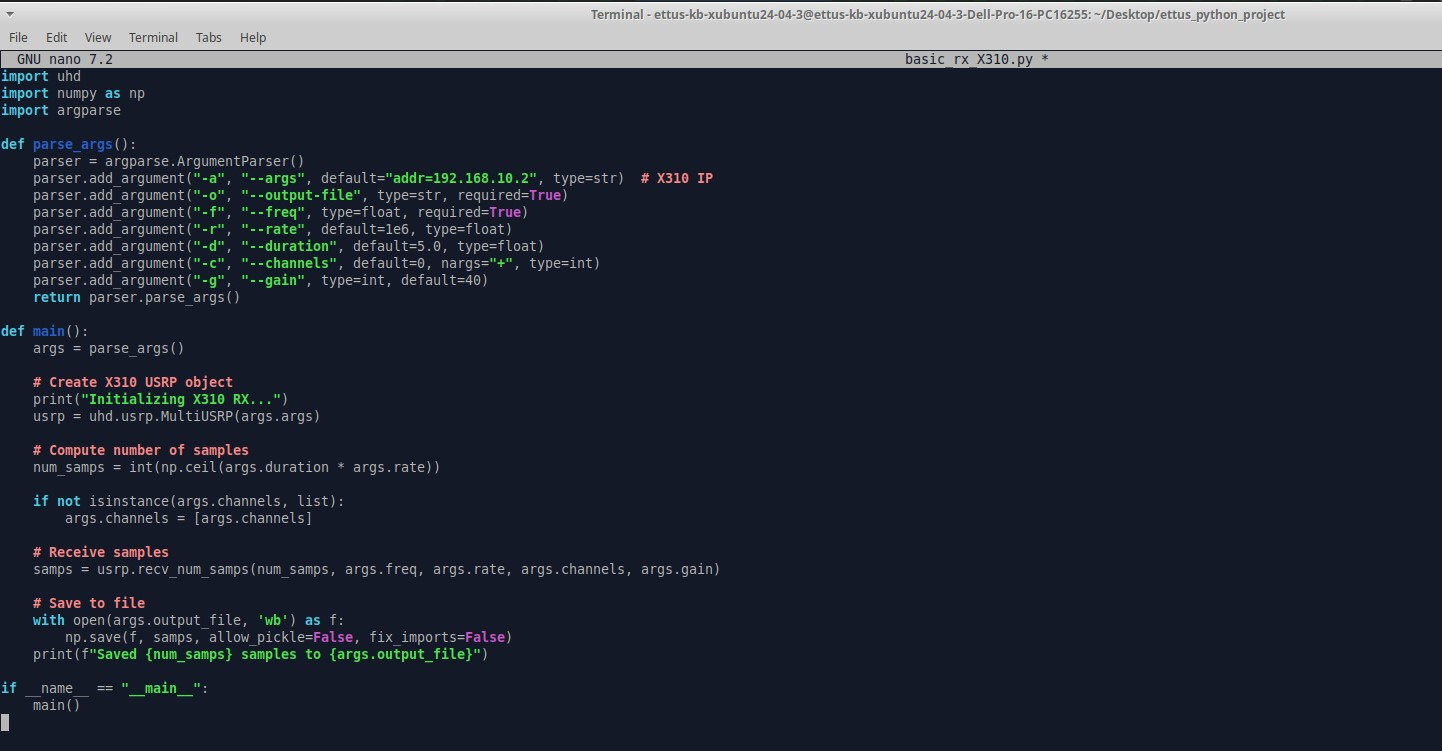
\includegraphics[width=0.95\linewidth,height=0.46\textheight,keepaspectratio]
{latex/jpg_png/image_python_api_X310_python code.jpg}
\end{center}

\end{frame}